\chapter{ランサムウェア}
% 本章では,本研究の提案手法に関連する要素に注目して,ランサムウェアについて説明する.





\section{概要}
\label{sec:ransom-overview}
ランサムウェアとはマルウェアの一種であり,攻撃者が要求した金額が支払われるまで,システムやデータへのアクセスを制限する.
言い換えると,データや計算資源,サービスなどのリソースを人質に取って被害者を脅迫することで身代金を要求するマルウェアがランサムウェアである.

ランサムウェアはリソースへのアクセスを制限する方法に基づいて暗号化ランサムウェアとロッカーランサムウェアに分類される \cite{oz2022survey}.
暗号化ランサムウェアは感染先ホストのファイルやデータを暗号化し,元のファイルを削除または上書きする.
ロッカーランサムウェアは暗号化を行わず,デスクトップのスクリーンやブラウザをロックすることで被害者がシステムを利用できないようにする.
本研究は暗号化ランサムウェアを対象としているため,本稿では暗号化ランサムウェアを単に「ランサムウェア」と呼ぶことにする.

\begin{figure}[t]
  \begin{center}
    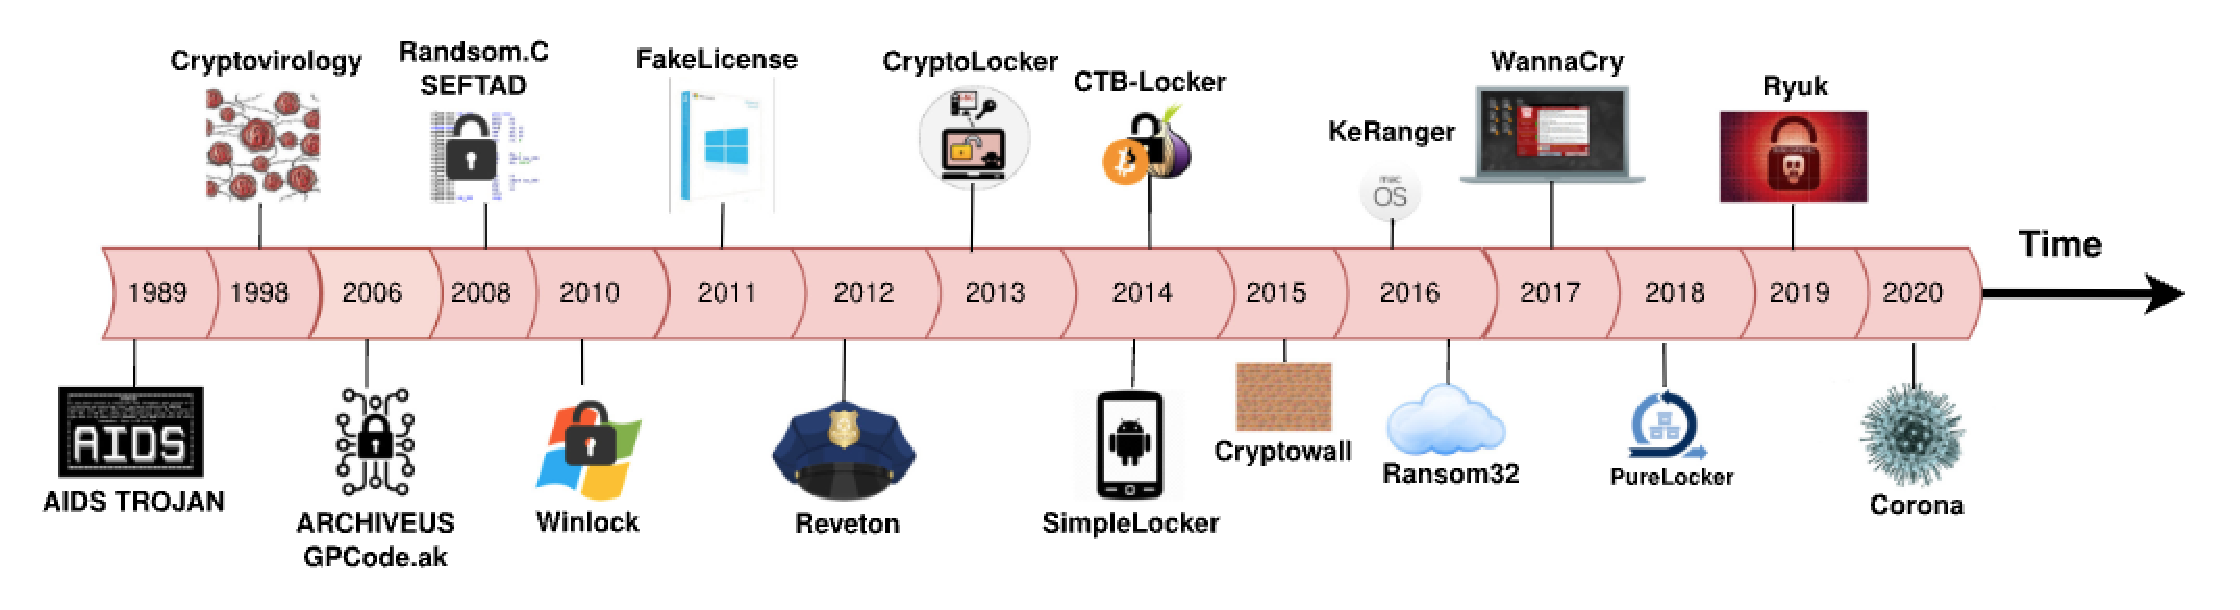
\includegraphics[width=\columnwidth]{doc/img/ransom-evolution.eps}
  \end{center}
  \caption{Development of major ransomware families (1989–2021). The first know ransomware, AIDS Trojan, was introduced in 1989. \cite{Evolution-Ransomware}.}
  \label{fig:ransom-evolution}
\end{figure}

\figref{fig:ransom-evolution}に示すように,AIDS Trojan \cite{aids-trojan} は1989年に最初のランサムウェアとして登場した.
AIDS Trojanは被害者に郵送されたフロッピーディスクを介して感染し,Windowsシステムを対象としていた.
その後インターネットの普及に伴い,ランサムウェアによる被害が増加し始めた.
2005年に登場したGPCode \cite{PGPCoder42:online} はフィッシングメールを介して感染し,独自の暗号化アルゴリズムによってファイルを暗号化した.

現代のランサムウェアはますます高度化している.
ランサムウェアの進化における重要な要素を以下に列挙する.
\begin{itemize}
  \item AESなどの対称鍵暗号化アルゴリズムやRSA,楕円曲線暗号などの非対称鍵暗号化アルゴリズムを使用して暗号化を行うようになっている \cite{Evolution-Ransomware}.
        これにより,復号鍵を入手することができなければデータの復号はほぼ不可能となった.

  \item Windowsだけでなく,Linux,macOS,Androidなどの他のOSを対象としたランサムウェアも登場するようになった.

  \item ビットコインに代表される仮想通貨が普及したことで身代金の支払いが匿名で行えるようになり,攻撃者の特定が難しくなった.

  \item ランサムウェアの開発と配布を有料で行うサービスであるRansomware as a Service (RaaS) が登場し,専門知識が無くとも容易に攻撃を実施することができるようになった.

  \item 無差別的な攻撃から,特定の高価値な組織 (政府機関や大企業など) を対象とした高度な攻撃に移行しつつある \cite{early-detection}.
\end{itemize}

\section{ランサムウェアの分類}
\subsection{悪意ある振る舞いに基づく分類}
\ref{sec:ransom-overview}節で述べたように,ランサムウェアは被害者が身代金を支払うまでリソースへのアクセスを制限するが,
アクセスを制限する方法には多様性が見られる.
本稿ではOzらの分類 \cite{Evolution-Ransomware} を参照し,その方法として\textbf{暗号化},\textbf{データ破壊},\textbf{データ窃取}を扱う.

暗号化:
ランサムウェアは暗号化鍵を用いてデータを暗号化し,元のデータを削除するか,暗号化後のデータで上書きする.
この時使用する鍵はランサムウェアの実行ファイルに埋め込まれているか,感染先ホスト上で生成されるか,C2サーバとの通信から取得されるかのいずれかである.
ファイルを暗号化するランサムウェアの中には,暗号化の対象とするファイルを限定するものも存在する.
例えばCTB-Locker \cite{ctb-locker} は,被害者にとってより高価値なファイルのみを暗号化するために,
.pdfや.zipなどの拡張子を持つファイルを暗号化対象としている.
また,Jigsaw \cite{byrne2017jigsaw} は10MB以下のファイルのみを暗号化する.
このように,ランサムウェアの一部は暗号化の対象とするファイルを限定することで,
ランサムウェアの活動が検出されるリスクを緩和している \cite{huang2017flashguard}と考えられる.

データ破壊:
破壊活動を目的としているがランサムウェアに擬態して攻撃者の意図を隠蔽しようとするマルウェアが確認されている.
例えば,2017年に発見されたNotPetya \cite{Petya-No22:online} は,ハードディスク全体を暗号化した後,
ビットコインの送金先として無効なアドレスを提示していた.
このアドレスはランダムに生成されており,攻撃者が金銭を回収する意図がないことから,
NotPetyaは破壊活動を目的として作成されたと考えられる \cite{Petya-No22:online}.
同様の攻撃として,暗号化を行わず,ランダムなデータでファイルを上書きするマルウェアを作成し使用することも可能である.
なお,このタイプのマルウェアの被害者は身代金を支払ってもリソースを復旧することができないが,
本研究ではランサムウェアとして扱う.

データ窃取:
ランサムウェアは機密文書や顧客の個人情報などの重要データを摂取する可能性がある.
データの暗号化または破壊とデータの窃取を組み合わせて脅迫を行うランサムウェアを「二重脅迫ランサムウェア」と呼ぶ.
二重脅迫ランサムウェアは,データの復旧のために一回,窃取したデータの公開を防ぐためにもう一回,被害者に身代金を要求する.
二重脅迫ランサムウェアによる被害は近年増加しており,SOPHOS社が発表したレポート \cite{sophos-report:online} によると,
2023年に発生したランサムウェアインシデントのうち32\%においてデータの摂取も発生している.
加えて,データの窃取のみによって脅迫を行う「ノーウェアランサム」\cite{nowhere-ransom} と呼ばれる手法も確認されている.

\subsection{暗号化アルゴリズムに基づく分類}
データを暗号化するランサムウェアは,ISO/IEC \cite{ISOIEC2784:online} などの標準化団体が採択した標準的なアルゴリズムを使用する場合と,
攻撃者によって独自に設計された暗号化アルゴリズムを使用する場合がある.
Begovicら \cite{begovic2023cryptographic} が調査した,1991年から2021年までに確認された著名なランサムウェア変種の
暗号化アルゴリズムの使用状況を\figref{fig:encrypt_algo}に示す.
\figref{fig:encrypt_algo}によると8.2\%のランサムウェアが独自の暗号化アルゴリズムを使用しているが,
近年のランサムウェアはAESやRSAといった標準的な暗号化アルゴリズムを使用する傾向が強いことがいくつかの先行研究 \cite{Evolution-Ransomware,key-management}にて指摘されており,
この数値には初期のランサムウェアが多く含まれていると考えられる.
より具体的には,攻撃者が独自に設計した暗号化アルゴリズムは強度が不十分で暗号解読者による解読が容易であることが多い \cite{key-management}ため,
2000年代後半から2010年代前半にかけて,十分に評価され強度が高い暗号化アルゴリズムが採用されるようになっていった \cite{Evolution-Ransomware}.

\begin{figure}[tb]
  \begin{center}
    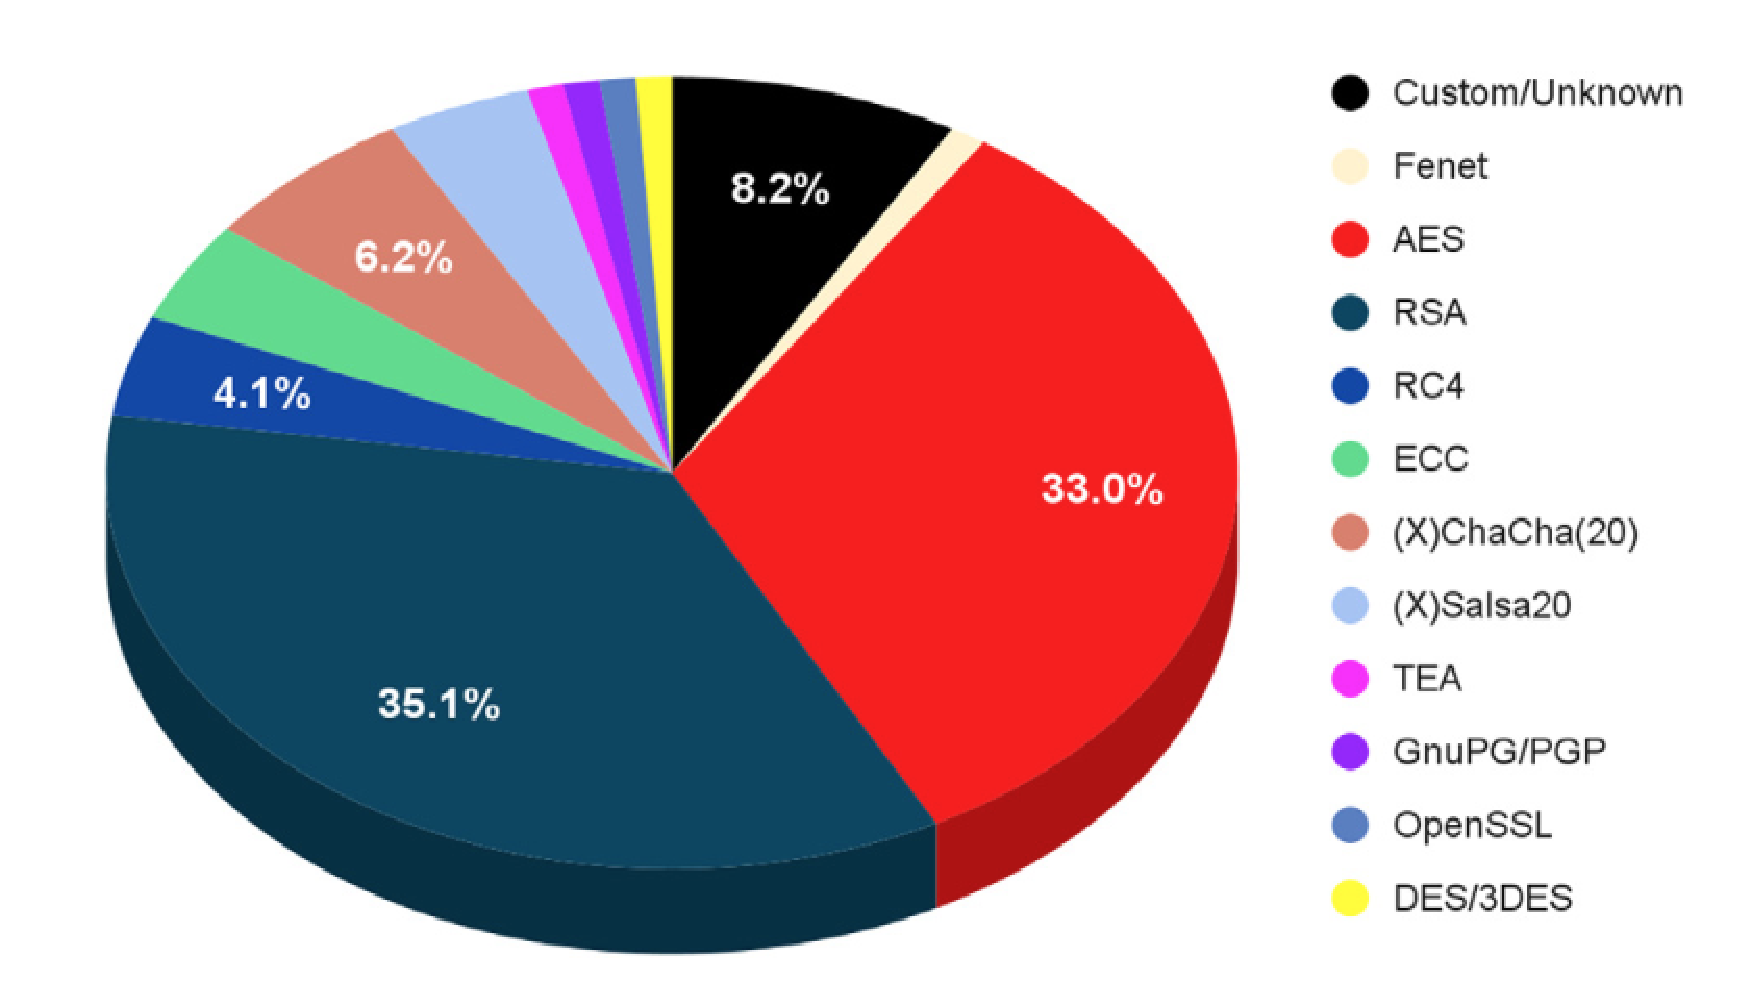
\includegraphics[width=0.8\columnwidth]{./doc/img/encrypt_algo.eps}
  \end{center}
  \caption{Breakdown of encryption algorithms used by major ransomware families (1989–2021). \cite{begovic2023cryptographic}}
  \label{fig:encrypt_algo}
\end{figure}

ランサムウェアは\textbf{対称鍵暗号化},\textbf{非対称鍵暗号化},\textbf{ハイブリッド暗号化}のいずれかの暗号化技術を採用することができる.
\\
対称鍵暗号化:
対称鍵暗号化では,暗号化と復号のために1つの鍵のみが使用される.
非対称鍵暗号化よりも高速に暗号化を行うことができるが,被害者が鍵を入手してファイルを復号することができる可能性がある.
例えば,PayBreak \cite{kolodenker2017paybreak} は,暗号化機能を提供するWindows APIの関数をフックして
暗号化に使用される共通鍵を取得することで復号を可能にしている.
そのため攻撃者は,鍵が被害者からアクセスできないようにする必要がある.
\figref{fig:encrypt_algo}より,ランサムウェアが採用する対称鍵暗号化アルゴリズムとしてはAESが
最も人気であることがわかる.
\\
非対称鍵暗号化:
非対称鍵暗号化では,暗号化鍵 (公開鍵) と復号鍵 (秘密鍵) の2つの鍵が使用される.
被害者が公開鍵を入手しても暗号化されたデータを復号することはできないため,対称鍵暗号化に比べて暗号化速度は劣るが,
暗号化鍵の保護を行う必要がない.
常に同一の鍵ペアを使用する場合,一度秘密鍵が漏洩 (または,ある被害者が身代金を支払って秘密鍵を取得)すると,その鍵ペアで暗号化されたデータは全て解読可能となる.
そのためCryptoLocker \cite{liao2016behind}などの一部のランサムウェアは,被害者ごとに異なる鍵ペアを生成する戦略を採用している.
RSAが最も頻繁に,楕円曲線暗号が次いで使用されていることが\figref{fig:encrypt_algo}よりわかる.
\\
ハイブリッド暗号化:
ハイブリッド暗号化では,
対称鍵暗号を用いてデータを暗号化した後,その暗号化鍵を非対称鍵暗号化アルゴリズムを用いて暗号化する.
これにより大量のデータの暗号化を効率よく実行しつつ,対称鍵暗号化における問題点であった鍵の保護を解決することができる.
近年の著名なランサムウェアはハイブリッド暗号化を採用しているものが非常に多い \cite{begovic2023cryptographic}.
代表例としてはWannaCry \cite{WannaCry} やCTBLocker \cite{ctb-locker} が挙げられる.

\subsection{暗号化の対象に基づく分類}
ランサムウェアはOS上でユーザが扱うデータファイル (e.g. .docx, .xlsx, .jpg) を暗号化することが一般的であるが,
ファイル以外の単位で暗号化を行うランサムウェアも存在する.
Mamba \cite{mamba-petya} はハードディスク全体を暗号化したのち
マスターブートレコード (MBR) を書き換えてOSの正常な起動を阻害し,OS起動時にランサムノートが表示されるようにする.
また,Petya \cite{mamba-petya} はWindowsシステムのマスターファイルテーブル (MFT)
\footnote{MFTはWindowsシステム内に存在するファイルの物理的な位置,ファイル名,作成者などのメタデータを管理するデータ構造である.}
を暗号化することでファイルのアクセスを不可能にする.
DarkSide \cite{DarkSide42:online} ランサムウェアはVMWare ESXi \cite{VMwarevS52:online}
のホストマシン上で実行される.DarkSideは実行中の仮想マシン (VM) を強制終了させ,VMの仮想ディスクなどの関連ファイルを暗号化する.
これらのファイルは,典型的には\texttt{/vmfs/volumes}ディレクトリ以下のファイルであるが,
仮想マシンからは認識できない.

今日のクラウドサービスの隆盛に伴い,クラウド環境を対象としたランサムウェア攻撃が増加している.
ALIBABA Cloudの仮想ストレージサービスは2023年の第三四半期のみで1000件以上の被害報告をユーザから受けており,
2021年と比較して118\%の増加率を示している \cite{wang2024ransom}.
さらにZscaler社  は,クラウドサービスやクラウド上のワークフローに最適化されたランサムウェア
が開発されることを予測\cite{zscaler-ransomware}しており,
新しいタイプのランサムウェアの出現に備える必要がある.

\section{ランサムウェアの影響}
% \subsection{発生する影響の種類}
% ランサムウェア攻撃を受けた組織には,以下のような影響が発生する可能性がある.
% \\
\subsection{データ損失}
ランサムウェアによって利用不可能になったデータは,攻撃者に身代金を支払ったとしても復旧される保証はない.
SpyCloud社のレポート \cite{spycloud-ransomware} (\figref{fig:pay-ransom-back-data}) によると,
2024年にランサムウェア攻撃者に対して身代金を支払った組織のうち,暗号化されたデータを完全に復旧することができたのは約50\%である.

攻撃者によって復旧の手段が提供されない場合でも,定期的なバックアップを取得していればデータ損失を緩和することが可能である.
しかしその場合でも,最新のバックアップからランサムウェア攻撃が発生するまでの間に更新されたデータは失われる\cite{wang2024ransom}.
さらにバックアップデータも侵害するランサムウェア攻撃が確認されている \cite{spycloud-ransomware}.
% % 定期的なバックアップの取得はデータの復旧を行うための有効な手段であるが,
% バックアップを定期的に取得していたとしても,
\begin{figure}[t]
  \begin{center}
    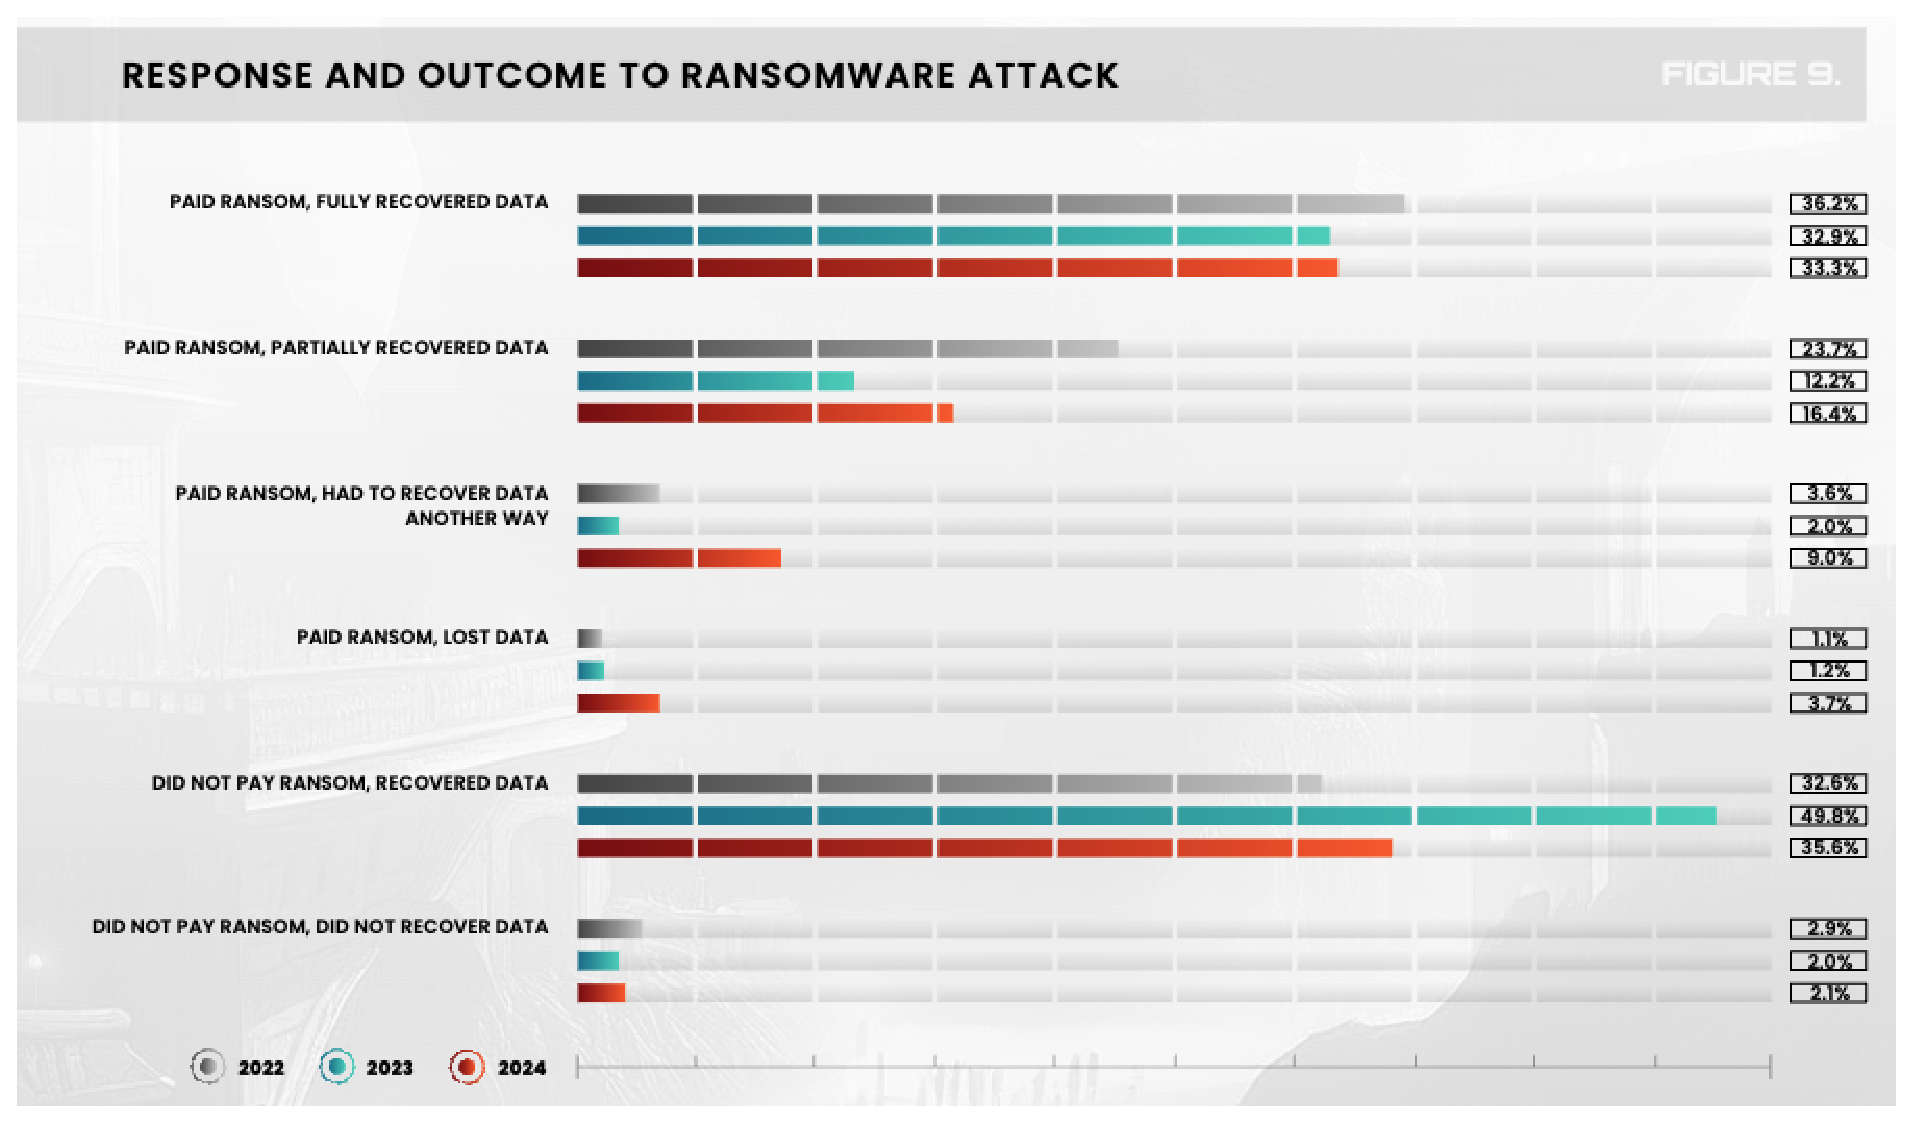
\includegraphics[width=\columnwidth]{doc/img/pay-ransom-back-data.eps}
  \end{center}
  \caption{
    This figure illustrates the outcomes of ransomware attacks based on whether victims paid the ransom and the success rate of data recovery.
    It categorizes results into fully recovered data, partially recovered data, recovery through alternative means, lost data despite paying, and outcomes for those who did not pay.
    The percentages are shown for the years 2022, 2023, and 2024. \cite{spycloud-ransomware}}
  \label{fig:pay-ransom-back-data}
\end{figure}


\subsection{金銭的損失}
攻撃者に支払う身代金がコストとして発生する.
さらに,システムダウンやデータアクセスの制限により,業務が停止することで本来のサービスが提供できなくなるためサービスのダウンタイム中に機会損失が発生するほか,
復旧作業の費用 (データ復旧,セキュリティ対策や調査の人件費,デバイスやネットワークの修理費用など) も生じる.

ランサムウェア攻撃の対象は無差別な個人から高価値な組織へと移行しつつあり,それに伴って身代金額も増加している.
SOPHOS社のレポート \cite{sophos-report:online} によると,
要求される身代金の中央値が200万USD,63\%が100万USD以上であり,30\%が500万USD以上であった.
同レポートの調査対象において身代金の中央値と平均値が最も高かったのはアメリカ合衆国中央政府であった.

\figref{fig:recovery-cost}に示すように,身代金の支払いを除く復旧コストは2024年に大幅な増加が確認された.
復旧コストの平均値は2023年の182万USDから273万USDに増加し\cite{sophos-report:online,spycloud-ransomware},
\figref{fig:recovery-cost}では年間の収益が中程度のグループにおいて復旧コストの増加が顕著である一方,
収益が高いグループではコストは微増または減少している.
% この結果は,高収益の企業はランサムウェア対策をはじめとするセキュリティ対策により
\begin{figure}[t]
  \begin{center}
    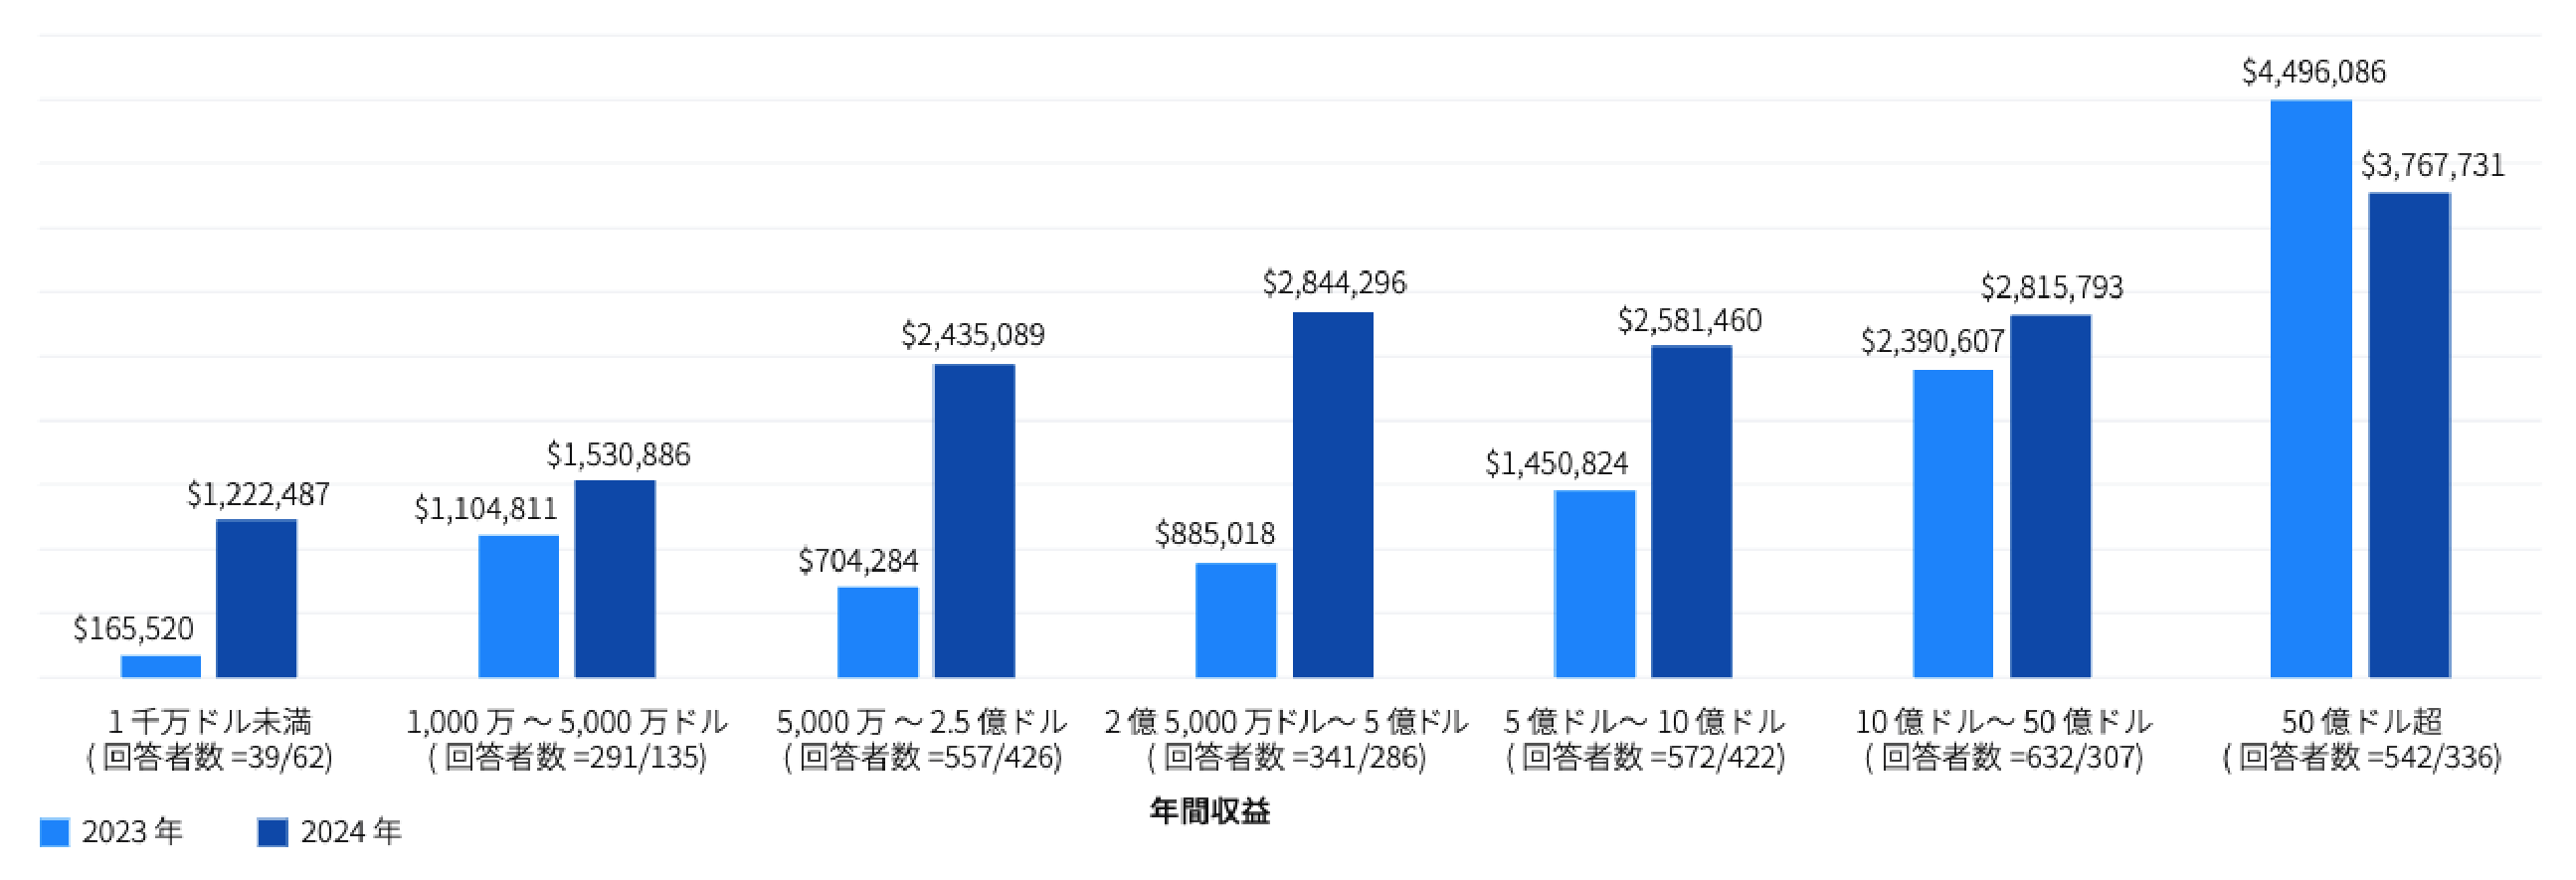
\includegraphics[width=\columnwidth]{doc/img/recovery-cost.eps}
  \end{center}
  \caption{Recovery costs from the most severe ransomware attacks in 2023 and 2024.
    The cost includes downtime, labor, device and network costs, and lost revenue. \cite{sophos-report:online}}
  \label{fig:recovery-cost}
\end{figure}

\subsection{信頼性の低下}
ランサムウェア攻撃を受けた企業は,データの保護やセキュリティへの投資が不十分であるとの印象を顧客や取引先に与えることがある.
これにより既存の顧客や取引先との取引関係が損なわれ,
逸失利益が発生する可能性がある.\figref{fig:recovery-cost}に示される復旧コストには逸失利益も含まれていることに注意する.
また非営利の組織であっても,メディア報道によってネガティブなイメージが拡散された結果
組織の活動に支障が出るおそれもある.

\subsection{長期的なリスク}
CyberReason社の調査 \cite{cyberreason-report}によると,ランサムウェア攻撃を受けて身代金を支払った企業は,その8割が
再度ランサムウェア攻撃を受ける.
したがって身代金支払いによって一度の攻撃に対処したとしても,その後も継続的に攻撃の対象となるリスクがある.

\section{主要なランサムウェアインシデント}
\subsection{WannaCryの事例 (2017年)}
ランサムウェアWannaCryによる攻撃は2017年5月に発生したランサムウェアインシデントである,
WannaCryはWindowsサーバの任意コード実行脆弱性 (CVE-2017-0143) を利用して,Microsoftによる脆弱性修正パッチが適用されていない
Windows7マシンを中心として感染を広げた.

スペインの大手通信事業者であるテレフォニカが最初の標的であり,その後ヨーロッパ諸国および世界中で感染が拡大して
最終的には100カ国以上で被害が発生した \cite{wannacry-attack}.
英国におけるNHS (National Health Service,国民保健サービス) の被害は特筆すべきものであり,
NHS全体で19,000件以上の来院予約のキャンセルと9200万ポンドの損失が生じ,
手術や診察の中止により人名にかかわる被害も報告された \cite{kaspersky-wannacry}.

\subsection{コロニアル・パイプライン社への攻撃 (2021年)}
RaaSを提供する犯罪者グループであるDarkSide \footnote{DarkSideという名前は犯罪者グループだけでなく,彼らが作成したランサムウェア \cite{DarkSide42:online}
  も指すが,本節では犯罪者グループを指す.}
は,VPNシステムの認証の不備をついてコロニアル・パイプライン社のネットワークに侵入し,ランサムウェア攻撃を展開して
データの窃取と暗号化を行った\cite{colonial-pipeline-attack}.
コロニアル・パイプライン社はランサムウェア攻撃を受けて一時的にパイプラインの操業を停止した.
同社はアメリカ合衆国の東海岸にて石油製品のパイプラインを運営しており,
インシデント発生当時には東海岸にて45\%の燃料供給を担っていたため,
操業停止の発表によってパニック的なガソリンの買い占めが発生し,一部の給油所で備蓄が枯渇した.
このインシデントで影響を受けたのは同社の社内ITシステムのみであったため輸送パイプラインは1週間以内に
稼働を再開することができたが,
パイプライン制御システムが攻撃されていた場合操業停止が長引いて燃料のサプライチェーンに深刻な影響を及ぼす可能性があった.

\subsection{名古屋港への攻撃 (2023年)}
2023年7月4日に,名古屋港のコンテナターミナルシステムを対象としたランサムウェア攻撃が発生し,
名古屋港の全ターミナルが約3日間作業停止となる障害が発生した\cite{nagoya-port-attack}.
名古屋港は総貨物取扱量や貿易額などの項目で日本一 \cite{nagoya-port-no1} であり,
復旧までに約2万本のコンテナの輸出入に影響が発生した.

本インシデントではコンテナターミナルシステムが稼働するすべての物理マシンおよび仮想マシン上のデータが暗号化され,
システムバックアップによる復旧が行われた.
ただしログはバックアップの対象外であり復旧作業中にログが消失したため,感染経路や感染の原因は特定されていない.

\subsection{株式会社KADOKAWAへの攻撃 (2024年)}
株式会社KADOKAWAは2024年6月にランサムウェア攻撃を受けたことを発表し,
動画配信サービスをはじめとする主要サービスの一部が一時的に停止した\cite{kadokawa-apology}.
この攻撃の対象は株式会社ドワンゴが使用するファイルサーバであり,ファイルの暗号化のみならずデータ窃取も行われた.
その結果,株式会社ドワンゴの従業員やユーザなど,合計で25万人以上の個人情報が流出したとされる.
この個人情報データはBlackSuitというランサムウェア犯罪グループによってダークネット上のリークサイトに公開された \cite{kadokawa-leak-PPI}.
\begin{figure}[t]
  \begin{center}
    \includegraphics[width=0.8\columnwidth]{doc/img/BlackSuit-2024-06-27-060714.eps}
  \end{center}
  \caption{A post by BlackSuit detailing their alleged access to KADOKAWA’s networks, encryption of the infrastructure,
    and theft of 1.5TB of data. \cite{kadokawa-leak-PPI}}
  \label{fig:kadokawa-leak}
\end{figure}

